
\section{Bauteilversuche}

\subsection{Allgemeines}

Die Tabelle \ref{tab:Versuchsprogramm} gibt einen Überblick über die Bauteilversuche  und die Unterschiede im Aufbau. Grundlage für die Änderungen der Bauteilkomponenten waren der Gedanke die Material- und Herstellungskosten zu reduzieren. 

\begin{table}[h]
\caption{Versuchsprogramm}
\begin{center}
\begin{tabular}{|c|c|c|c|c|}
\hline 
\multicolumn{5}{|c|}{ Übersicht} \\ 
\hline 
Versuch & Abmessungen  & Schraubenanzahl & Kleber & Aushärtezeit \\ 

&  l x b x h in [m] & (Fa. SFS) & (Fa. Sika)   & Tage \\ 
\hline\hline
1 & 7,40 x 0,50 x 0,33 & 28 & Sikadur 31   & 14 \\ 
\hline 
2  & 7,40 x 0,50 x 0,33 & 8 & ElastoCem 109  & 21 \\ 
\hline 
3 & 7,40 x 0,50 x 0,33 & 12 & Sikatop 107  & 28 \\ 
\hline 
4  & 7,40 x 0,50 x 0,33 & - & Sikatop 107  & 28 \\ 
\hline 
\end{tabular} 
\end{center}
\label{tab:Versuchsprogramm}
\end{table}

\subsection{Bauteilversuch\,1\,(BT\,1)}

\subsubsection{Versuchskörper}

Der grundsätzliche Schichtenaufbau ist in Abschnitt 2.1.2 beschrieben. 

 Die Anordnung der Schrauben ist der Abbildung \ref{1versuch} zu entnehmen. Die Schrauben wurden analog zum Verlauf der Querkraftlinie zufolge einer Gleichlast angeordnet, d.h.\ im Auflagerbereich ist der Schraubenabstand geringer als in Trägermitte. Es wurde zwischen der Holz und Holzbetonschicht sowie zwischen den Holzbetonschichten der Kleber SikaDur 31-A Normal verwendet. 
 
  Die Durchbiegungen wurden an den Rändern des Trägers gemessen. 
Um eine auftretende Torsion während des Versuchs erfassen zu können, wurden in der Trägermitte zwei Messuhren an den Ränders angebracht.


\begin{figure}[h!]
\begin{center}
\includegraphics[scale =0.9,trim= 1.5cm 10cm 1.5cm 10cm, clip=true]{Auswertung/1versuch/BT1.pdf}
\caption{Darstellung des BT\,1, mit Verbindungsmittel und Lasteinleiung}
\label{1versuch}
\end{center}
\end{figure}

\subsubsection{Versuchsablauf}

Der Versuch wurde manuell kraftgesteuert durchgeführt, die Belastungsgeschwindigkeit betrug etwa \unit[4]{kN/min}. Bei der Laststufe von \unit[58]{kN} (je Zylinder) wurde ein Haltepunkt eingefügt, da eine Keilzinkung versagte (Abbildung \ref{keilzinkung}). 

Bei weiterer Belastung wurde die Maximallast von \unit[78]{kN} erreicht. Nach dieser Laststufe erhöhte sich die Durchbiegung sprunghaft bei gleichzeitiger Reduktion der aufgebrachten Last.

Um einen vollständigen Bruch des Systems herbeizuführen, wurde der Bauteil nochmals belastet. Der Bruch trat bei einer Last von \unit[48]{kN} ein (Abbildung \ref{1bruch}).

\subsubsection{Versagensbeschreibung}

Das erste Versagen wurde bei einer Last von \unit[58]{kN} festgestellt. Unter $F_{A}$ brach eine Keilzinkung der Brettsperrholzplatte. In Abbildung \ref{keilzinkung} ist der Schaden am Bauteil darstellt. Im Diagramm in Abbildung \ref{1_versuch_kraft_schubverschiebung} ist zu erkennen, dass vor dem erreichen dieser Laststufe bereits eine erhöhte horizontale Verschiebung zwischen Beton und Holz bei Auflager A stattfand. 

Das Versagen der Klebefuge führte zu einer Spannungsumlagerung in den Teilquerschnitten Beton und Holz. 
Durch die aus der Spannungsumlagerung erhöhten Randspannungen brach die Keilzinkung unter dem Lasteinleitungspunkt $F_{A}$(Abbildung \ref{keilzinkung}).  
  
Beim weiteren Belasten waren Risse im Beton zwischen der Kraft $F_{A}$ und dem Auflager A entstanden. Die maximale Belastung betrug \unit[78]{kN}. 



Durch den Bruch konnte danach die Fuge zwischen Holzspanbeton und Holz betrachtet werden (Abbildung \ref{bruchbild}). Es zeigte sich, dass ca.\ ein Viertel der Fläche ungenügenden Verbund hatte. Ein Grund für das Versagen der Verbundfuge dürfte in der ungenügenden Vernetzung der Klebeschicht zwischen Holz und Holzbeton liegen. Durch den unzureichenden Verbund kam es zu höheren Biegespannungen in den Teilquerschnitten Holz und Beton und damit zum Bruch der Keilzinkung.

Desweiteren wurde ersichtlich, dass in diesem Bereich des Trägers zwei Schrauben nicht aus dem Holz ausgezogen wurden, sondern in der Klebefuge zwischen Holz und Holzbeton abgerissen sind. Die restlichen Schrauben wurden aus der Brettsperrholzplatte ausgezogen. 




\begin{figure}[h!]
\begin{minipage}[hbt]{7cm}
	\includegraphics[width=7cm]{Auswertung/1versuch/keilzinkung.png}
	\caption{Versagen der Keilzinkung unter der Lasteinleitung $F_{A}$ }
	\label{keilzinkung}
\end{minipage}
\hfill
\begin{minipage}[hbt]{7cm}
	\includegraphics[width=7cm]{Auswertung/1versuch/Betonriss78kN.jpg}
	\caption{Betonriss im Bereich der Krafteinleitung $F_{A}$ nach Maximalbelastung }
	\label{1bruch}
\end{minipage}
\end{figure}
 


\begin{figure}[h!]
\begin{minipage}[hbt]{7cm}
	\includegraphics[width=7cm]{Auswertung/1versuch/bruch_1versuch.png}
	\caption{Bruch nach Wiederbelastung }
	\label{1bruch}
\end{minipage}
\hfill
\begin{minipage}[hbt]{7cm}
	\includegraphics[width=7cm]{Auswertung/1versuch/bruchbild.png}
\caption{Bruchbild der BSP-Platte }
	\label{bruchbild}
\end{minipage}
\end{figure}

\subsubsection{Verformungsverhalten}

In Abbildung \ref{1 Versuch: Kraft-Durchbiegung} ist die Arbeitslinie des Versuchs dargestellt.

Sie weist einen annähernd linearen Verlauf bis zu der Kraft von \unit[58]{kN} auf. Wie im Diagramm ersichtlich, besteht kein Unterschied zwischen den Messpunkten  u\,1.1 und u\,1.2, d.h.\ es kam zu keiner Torsion während des Versuch.
Der weitere Verlauf der Kennlinie ist mit einigen Knicken versehen, die als Datenerfassungsfehler interpretiert werden. 

Abbildung \ref{1_versuch_kraft_schubverschiebung} zeigt die relative Verschiebung zwischen der BSP-Schicht und der Betonschicht. Bis zur Laststufe von \unit[35]{kN} trat keine messbare Verschiebung auf. Weiters ist erkennbar, dass bei \unit[58]{kN} der Verbund zwischen der BSP-Schicht und der Holzbetonschicht nicht mehr vorhanden war. 

Die Abflachung der Kurve zwischen \unit[58] und \unit[60]{kN} beinhaltet die Kriechverformung zufolge der konstant gehaltenen Kraft von \unit[58]{kN}(siehe auch Abbildung \ref{1 Versuch: Kraft-Durchbiegung-Zeit}). Während die Kurve u\,4 (Verschiebung bei Auflager B) bei weiterer Belastung die gleiche Steigung wie vor dem Haltepunkt aufweist, zeigt die Kurve u\,5 das fortschreitende Versagen der Schubverbindungen zwischen Beton und Holz. 


\begin{figure}[h!]
\begin{center}
\begin{tikzpicture}
\begin{axis}[height=12cm, width=12cm, 
			no markers,
			xmajorgrids,ymajorgrids,
			ylabel=Kraft\,/\,Zylinder\,$\lbrack kN\rbrack$,
			xlabel=Verschiebung\,u\,$\lbrack mm\rbrack$,
			xmin=0,ymin=0,
			legend pos=south east			
			 ]
\addplot table[y=F,x=u1.1]{Auswertung/1versuch/BT1.dat};
\addplot table[y=F,x=u1.2]{Auswertung/1versuch/BT1.dat};
\addplot table[y=F,x=u2]{Auswertung/1versuch/BT1.dat};
\addplot table[y=F,x=u3]{Auswertung/1versuch/BT1.dat};
\legend{BT1\,u1.1,BT1\,u1.2,BT1\,u2,BT1\,u3};
\end{axis}
\end{tikzpicture}
\caption{Bauteilversuch 1: Kraft-und Verschiebungsverlauf}
\label{1 Versuch: Kraft-Durchbiegung}
\end{center}
\end{figure}

\begin{figure}[h!]
\begin{center}
\begin{tikzpicture}
\begin{axis}[height=12cm, width=12cm,
			axis y line*=left, 
			no markers,
			xmajorgrids,ymajorgrids,
			xlabel=Zeit\,$\lbrack s \rbrack$,
			ylabel=Kraft\,/\,Zylinder\,$\lbrack kN\rbrack$,
			xmin=0,ymin=0,
			legend pos= north east			
			 ]
\addplot table[y=F,x=t]{Auswertung/1versuch/BT1.dat};
\legend{F};
\end{axis}
\begin{axis}[height=12cm, width=12cm, 
			axis y line*=right,
			axis x line*=none,
			no markers,
			xmajorgrids,ymajorgrids,
			ylabel=Verschiebung\,u\,$\lbrack mm\rbrack$,
			xmin=0,ymin=0,
			legend pos=south east			
			 ]
\addplot table[y=u1.1,x=t]{Auswertung/1versuch/BT1.dat};
\addplot table[y=u1.2,x=t]{Auswertung/1versuch/BT1.dat};
\addplot table[y=u2,x=t]{Auswertung/1versuch/BT1.dat};
\addplot table[y=u3,x=t]{Auswertung/1versuch/BT1.dat};
\legend{BT1\,u1.1,BT1\,u1.2,BT1\,u2,BT1\,u3};
\end{axis}
\end{tikzpicture}
\caption{Bauteilversuch 1: Kraft-und Verschiebungsverlauf in Abhängigkeit von der Zeit}
\label{1 Versuch: Kraft-Durchbiegung-Zeit}
\end{center}
\end{figure}




\begin{figure}[h!]
\begin{center}
\begin{tikzpicture}
\begin{axis}[height=12cm, width=12cm,
			no markers,
			xmajorgrids,ymajorgrids,
			xlabel=Verschiebung\,u\,$\lbrack mm \rbrack $,
			ylabel=Kraft\,/\,Zylinder\, $\lbrack kN \rbrack $,			
			xmin=0,ymin=0,
			legend pos= south east
			 ]
				\addplot table[y=F,x=u4]{Auswertung/1versuch/BT1.dat};
				\addplot table[y=F,x=u5]{Auswertung/1versuch/BT1.dat};
				\legend{BT1\,u4,BT1\,u5}
\end{axis}
\end{tikzpicture}
\caption{Bauteilversuch 1: Kraft-Schubverschiebung}
\label{1_versuch_kraft_schubverschiebung}
\end{center}
\end{figure}



\clearpage
 
\subsection{Bauteilversuch\,2\,(BT\,2)}

\subsubsection{Versuchskörper}

Der grundsätzliche Schichtenaufbau ist in Abschnitt 2.1.2 beschrieben.

Im Unterschied zum Versuch BT\,1 (ref) wurden die Schrauben analog zum Querkraftverlauf zufolge der  Belastungsanordnung im Versuch positioniert. Mittels einer Finite Elemente Berechnung mit dem Programm Sofistik wurde die Lage der Schrauben so optimiert, dass die Schrauben die gleiche Normalkraft erfahren. 



Nach den Kleberversuchreihe\,1(ref) wurde der Kleber ElastoCem 109 verwendet.


\paragraph{Schädigungen vor Versuchsdurchführung}
\label{abs:BT2_Schaden}

Die Schädigungen sind beim Einheben des Trägers in die Prüfanlage aufgetreten. Der Träger wurde mit zwei Gurten, die im einem Abstand von\unit[3]{m} zueinander in der Mitte des Trägers befestigt wurden, angehoben. Durch den daraus resultierenden Lastzustand entstanden die Betonzugrisse im Abstand von ca.\ \unit[150]{cm} von den Trägerenden (Abbildung \ref{schädigung scc}) und der Spalt in der obersten Klebefuge an den Trägerenden (Abbildung \ref{schädigung velox}).

Über die gesamte Länge des Träger wurden außerdem in der obersten Kleberfuge ungenügende Vernetzungen im Randbereich der einzelnen Veloxplatten festgestellt. An diesen Stellen war jeweils ein deutlicher Spalt zwischen den Veloxschichten zu sehen. 

Entgegen der Resultate der Kleberversuchsreihe\,1 erwiesen sich die Eigenschaften des hier verwendeten Kleber als ungeeignet für das Sandwichsystem. 



\subsubsection{Versuchsablauf}

Der Versuch wurde ebenfalls manuell kraftgesteuert durchgeführt. 
Die Belastungsgeschwindigkeit betrug etwa \unit[4]{kN/min}.  

Die Maximalkraft betrug \unit[31]{kN}. Danach fiel die Belastung auf \unit[18]{kN} ab, als der maximale Zylinderweg der Prüfanlage erreicht wurde.
Um einen vollständigen Bruch des Systems herbeizuführen, wurde der Bauteil nochmals belastet. Der Bruch trat bei einer Last von \unit[21]{kN} ein ).



\begin{figure}[h!]
\begin{center}
\includegraphics[scale =0.9,trim= 1.5cm 10cm 1.5cm 10cm, clip=true]{Auswertung/2versuch/BT2.pdf}
\caption{Darstellung des BT\,2, mit Verbindungsmittel und Lasteinleiung}
\label{1versuch}
\end{center}
\end{figure}



\begin{figure}[h]
\begin{minipage}[hbt]{7cm}	
	\includegraphics[width=7cm]{Auswertung/2versuch/schädigung_velox.jpg}
	\caption{Schädigung beim Auflager B}
	\label{schädigung velox}
\end{minipage}
\hfill
\begin{minipage}[hbt]{7cm}
	\includegraphics[width=7cm]{Auswertung/2versuch/schädigung_scc.jpg}
	\caption{Schädigung des Betons, bei $F_{B}$}
	\label{schädigung scc}
\end{minipage}
\end{figure}


\subsubsection{Versagensbeschreibung}

Abschnitt \ref{abs:BT2_Schaden} beschreibt die Schädigungen, die durch das Einheben des Trägers in die Prüfanlage entstanden sind.  

Wegen des großflächig nicht vorhandenen Verbundes in den Klebefugen (Abbildung \ref{velos unten} und \ref{velox ober}) wird davon ausgegangen, dass die mechanischen Verbindungsmittel (Schrauben) alleine die Verbundwirkung zwischen Holz und Beton herstellen. 

Bei der Laststufe von \unit[24]{kN} fand das erste sichtbare Versagen in der Holzschicht statt. Es spaltete sich ein Keil in der Zugzone in Trägermitte ab (Abbildung \ref{2versuch versagen}).

Bei der Maximallast von \unit[31]{kN} versagten die Schrauben beim Auflager A durch Herausziehen aus 
dem Holz. Es zeigt sich bei Betrachtung der überproportionalen Relativverschiebung zwischen Holz- und Betonschicht (Abbildung \ref{BT2_Verschiebung_AuflagerA} ). 
\subparagraph{Anmerkung:} Die Verschiebung ist im Diagramm in Abbildung \ref{2_versuch_kraft_schubverschiebung} nicht erfasst, da die analogen Wegaufnehmer aus Sicherheitsgründen zu diesem Zeitpunkt bereits entfernt worden sind. 

Der vollständige Bruch der BSP-Platte fand  nach Wiederbelastung zwischen dem Lasteinleitungspunkt $F_{A}$ und Trägermitte bei einer Last von \unit[21]{kN} statt (Abbildung \ref{2versuch bruchbild}).




\begin{figure}
\begin{center}
\includegraphics[scale =0.1]{Auswertung/2versuch/BT2_Verschiebung_AuflagerA.jpg}
\caption{Horizontale Verschiebung beim Auflager A, nach Maximalbelastung}
\label{BT2_Verschiebung_AuflagerA}
\end{center}
\end{figure}


\begin{figure}
\begin{center}
\includegraphics[scale =0.5]{Auswertung/2versuch/2versuch_versagen.jpg}
\caption{Darstellung des Versagen}
\label{2versuch versagen}
\end{center}
\end{figure}


\begin{figure}
\begin{center}
\includegraphics[scale =0.1]{Auswertung/2versuch/BT2_bruchbild.jpg}
\caption{Darstellung des vollständigen Bruchs}
\label{2versuch bruchbild}
\end{center}
\end{figure}


\begin{figure}[h]
\begin{minipage}[hbt]{7cm}	
	\includegraphics[width=7cm]{Auswertung/2versuch/2versuch_1oberfläche_velox.jpg}
	\caption{Oberfläche der aufgetragenen Schicht}
	\label{velos unten}
\end{minipage}
\hfill
\begin{minipage}[hbt]{7cm}
	\includegraphics[width=7cm]{Auswertung/2versuch/2versuch_2oberfläche_velox.jpg}
	\caption{Oberfläche der aufgelegten Schicht}
	\label{velox ober}
\end{minipage}
\end{figure}

\subsubsection{Verformungsverhalten}


In Abbildung \ref{2 Versuch: Kraft-Durchbiegung} ist die Arbeitslinie des Versuchs dargestellt.


Der Verlauf der Arbeitslinien ist bis zu einer Last von \unit[14]{kN} linear. Danach nehmen die Verformungen progressiv zu. Über der Belastung von \unit[16]{kN} vergrößert sich der Unterschied zwischen der Verschiebungslinien u2 und u3. Es ist auf die Abspaltung des Holzkeils der BSP-Platte zurückzuführen (Abbildung \ref{2versuch versagen}). 
 

Die relative Verschiebung zwischen der BSP-Schicht und der Betonschicht ist in Abbildung \ref{2_versuch_kraft_schubverschiebung} darstellt. Die Arbeitslinien sind nahezu ident. Sie weisen bis zu \unit[15]{kN} ein lineares Verhalten auf, danach ist ein progressiver Anstieg erkennbar.


\begin{figure}[h!]
\begin{center}
\begin{tikzpicture}
\begin{axis}[height=12cm, width=12cm, 
			no markers,
			xmajorgrids,ymajorgrids,
			xlabel=Verschiebung\,u\,$\lbrack mm \rbrack $,
			ylabel=Kraft\,/\,Zylinder\,$\lbrack kN\rbrack $,
			xmin=0,ymin=0,
			legend pos= south east
			]
\addplot table[y=F,x=u1]{Auswertung/2versuch/BT2.dat};
\addplot table[y=F,x=u2]{Auswertung/2versuch/BT2.dat};
\addplot table[y=F,x=u3]{Auswertung/2versuch/BT2.dat};
\legend{BT2\,u1,BT2\,u2,BT2\,u3}
\end{axis}
\end{tikzpicture}
\caption{Bauteilversuch 2: Kraft-Durchbiegung}
\label{2 Versuch: Kraft-Durchbiegung}
\end{center}
\end{figure}





\begin{figure}[h!]
\begin{center}
\begin{tikzpicture}
\begin{axis}[height=12cm, width=12cm,
			axis y line*=left, 
			no markers,
			xmajorgrids,ymajorgrids,
			xlabel=Zeit\,$\lbrack s \rbrack$,
			ylabel=Kraft\,/\,Zylinder\,$\lbrack kN\rbrack$,
			xmin=0,ymin=0,
			ymax=30,
			legend pos= north east			
			 ]
\addplot table[y=F,x=Time]{Auswertung/2versuch/BT2.dat};
\legend{F};
\end{axis}
\begin{axis}[height=12cm, width=12cm, 
			axis y line*=right,
			axis x line*=none,
			no markers,
			xmajorgrids,ymajorgrids,
			ylabel=Verschiebung\,u\,$\lbrack mm\rbrack$,
			xmin=0,ymin=0,
			ymax=60,
			legend pos=south east			
			 ]
\addplot table[y=u1,x=Time]{Auswertung/2versuch/BT2.dat};
\addplot table[y=u2,x=Time]{Auswertung/2versuch/BT2.dat};
\addplot table[y=u3,x=Time]{Auswertung/2versuch/BT2.dat};
\legend{BT2\,u1,BT2\,u2,BT2\,u3};
\end{axis}
\end{tikzpicture}
\caption{Bauteilversuch 2: Kraft-und Verschiebungsverlauf in Abhängigkeit von der Zeit}
\label{1 Versuch: Kraft-Durchbiegung-Zeit}
\end{center}
\end{figure}

\begin{figure}[h!]
\begin{center}
\begin{tikzpicture}
\begin{axis}[height=12cm, width=12cm, 
			no markers,
			xmajorgrids,ymajorgrids,
			xlabel=Verschiebung\,u\,$\lbrack mm \rbrack $,
			ylabel=Kraft\,/\,Zylinder\,$\lbrack kN\rbrack $,
			xmin=0,ymin=0,
			legend pos= south east
			]
\addplot table[y=F,x=u4]{Auswertung/2versuch/BT2.dat};
\addplot table[y=F,x=u5]{Auswertung/2versuch/BT2.dat};
\legend{BT2\,u4,BT2\,u5}
\end{axis}
\end{tikzpicture}
\caption{Bauteilversuch 2: Kraft-Schubverformung}
\label{2_versuch_kraft_schubverschiebung}
\end{center}
\end{figure}






\clearpage

\subsection{Bauteilversuch\,3\,(BT\,3)}

\subsubsection{Versuchskörper}
\label{abs:BT3_Versuchskoerper}

Der Schichtenaufbau ist in Abschnitt 2.1.2 beschrieben. 

Aufgrund der Erfahrungen, die mit dem Bauteil BT\,2 gemacht wurden, wurden folgende Änderungen bei den Verbindungsmitteln vorgenommen.

Die Anzahl und Anordnung der Schrauben ist der Abbildung \ref{3versuch} zu entnehmen. Im Auflagerbereich wurde eine zusätzliche Schraube angeordnet, um den Lastfall`"Einheben des Versuchskörpers in die Prüfanlage'" zu berücksichtigen.  

Weiters wurde ein Kleber mit höherer Steifigkeit (Sikatop 107) eingesetzt (siehe Kleberversuchsreihe\,2).


\begin{figure}[h!]
\begin{center}
\includegraphics[scale =0.9,trim= 1.5cm 10cm 1.5cm 10cm, clip=true]{Auswertung/3versuch/BT3.pdf}
\caption{Darstellung des BT\,3, mit Verbindungsmittel und Lasteinleiung}
\label{1versuch}
\end{center}
\end{figure}

\subsubsection{Versuchsablauf}


Wie im Abschnitt \ref{abs:Versuchsbaufaufbau_Durchführung} beschrieben, wurde der Versuch mit einer digitalen Messeinrichtung versehen und mithilfe einer programmierten Belastungskurve gesteuert. Abbildung \ref{3 Versuch: Kraft-Durchbiegung-Zeit} zeigt den zeitlichen Ablauf des Versuchs. 

Bei der Last von \unit[35]{kN} wurde ein weiterer Haltepunkt mit einer Dauer von \unit[30]{min} eingefügt, um das kurzzeitige Kriechverhalten  unter hoher Last zu beobachten.

Anschließend wurde der Bauteil weiter belastet, bis ein deutlicher Lastabfall eintrat. Die Maximallast betrug \unit[58]{kN}.

Nach Entfernung der Messinstrumente wurde der Bauteil manuell gesteuert belastet, bis die BSP-Platte bei einer Last von \unit[35]{kN} im Bereich der Lasteinleitung $F_B$ brach.

 



 

\begin{figure}[h!]
\begin{minipage}[hbt]{7cm}	
	\includegraphics[width=7cm]{Auswertung/3versuch/beton_veloxriss.jpg}
	\caption{Darstellung des Risse im Beton und Holzbeton}
	\label{beton_veloxriss}
\end{minipage}
\hfill
\begin{minipage}[hbt]{7cm}
	\includegraphics[width=7cm]{Auswertung/3versuch/fuge.jpg}
	\caption{Spalt zwischen BSP und Holzbeton}
	\label{spalt}
\end{minipage}
\end{figure}


\begin{figure}
\begin{center}
	\includegraphics[scale=0.1]{Auswertung/3versuch/bruch_3versuch.jpg}
	\caption{Bruch nach Wiederbelastung bei Lasteinleitung $F_B$  }
	\label{bruch_3versuch}
\end{center}
\end{figure}




\begin{figure}
\begin{center}
	\includegraphics[width=6cm]{Auswertung/3versuch/fugenbruch_3versuch.jpg}
	\caption{Oberflächbild: BSP-Platte und Holzspanbeton}
	\label{fugenbruch_3versuch}
\end{center}
\end{figure}

\subsubsection{Versagensbeschreibung}

Die erste Schädigung trat als Riss im Beton und im Holzbeton im Bereich der Lasteinleitung $F_{B}$ bei der Maximallast von \unit[58]{kN} auf (Abbildung \ref{beton_veloxriss}). Dieser Betonzugriss ist ein Resultat der Spannungsumlagerung, welche sich zufolge des Versagens der Holzschrauben einstellt. Dieser Verlust der Verbundwirkung ist auch im Diagramm in Abbildung \ref{3 Versuch: Kraft-Schubverformung} zu sehen. Die Relativverschiebung zwischen Holz und Beton bei Auflager B (u4) erhöht sich im Bereich der Maximallast progressiv.

Abbildung \ref{fugenbruch_3versuch} zeigt eine gute Verklebung im Mittelbereich des Bauteils, hier versagte das Velox. In den Randbereichen versagte hingegen die Klebefuge. 


\begin{figure}
\begin{center}
\begin{tikzpicture}
\begin{axis}[	legend pos= south east,
				height=12cm, width=12cm,
				no markers,
				xmajorgrids,ymajorgrids,
				xlabel=Verschiebung\, u \,$\lbrack mm \rbrack $  ,
				ymin=0,xmin=0,
				ylabel=Kraft\, / \,Zylinder\, $\lbrack kN\rbrack $
				]
\addplot table[y=F,x=u1]{Auswertung/3versuch/BT3.dat};
\addplot table[y=F,x=u2]{Auswertung/3versuch/BT3.dat};
\addplot table[y=F,x=u3]{Auswertung/3versuch/BT3.dat};
\legend{BT3\,u1,BT3\,u2,BT3\,u3}
\end{axis}
\end{tikzpicture}
\caption{Bauteilversuch 3: Kraft-Durchbiegung}
\label{3 Versuch: Kraft-Durchbiegung}
\end{center}
\end{figure}


\begin{figure}[h!]
\begin{center}
\begin{tikzpicture}
\begin{axis}[height=12cm, width=12cm,
			axis y line*=left, 
			no markers,
			xmajorgrids,ymajorgrids,
			xlabel=Zeit\,$\lbrack s \rbrack$,
			ylabel=Kraft\,/\,Zylinder\,$\lbrack kN\rbrack$,
			xmin=0,ymin=0,
			ymax=60,
			legend pos= north east			
			 ]
\addplot table[y=F,x=Time]{Auswertung/3versuch/BT3.dat};
\legend{F};
\end{axis}
\begin{axis}[height=12cm, width=12cm, 
			axis y line*=right,
			axis x line*=none,
			no markers,
			xmajorgrids,ymajorgrids,
			ylabel=Verschiebung\,u\,$\lbrack mm\rbrack$,
			xmin=0,ymin=0,
			ymax=60,
			legend pos=south east			
			 ]
\addplot table[y=u1,x=Time]{Auswertung/3versuch/BT3.dat};
\addplot table[y=u2,x=Time]{Auswertung/3versuch/BT3.dat};
\addplot table[y=u3,x=Time]{Auswertung/3versuch/BT3.dat};
\legend{BT3\,u1,BT3\,u2,BT3\,u3};
\end{axis}
\end{tikzpicture}
\caption{Bauteilversuch 3: Kraft-und Verschiebungsverlauf in Abhängigkeit von der Zeit}
\label{3 Versuch: Kraft-Durchbiegung-Zeit}
\end{center}
\end{figure}





\begin{figure}
\begin{center}
\begin{tikzpicture}
\begin{axis}[	legend pos= south east,
				height=12cm, width=12cm,
				no markers,
				xmajorgrids,ymajorgrids,
				xlabel=Verschiebung\, u \,$\lbrack mm \rbrack $  ,
				ymin=0,xmin=0,
				ylabel=Kraft\, / \,Zylinder\, $\lbrack kN\rbrack $
				]
\addplot table[y=F,x=u4]{Auswertung/3versuch/BT3.dat};
\addplot table[y=F,x=u5]{Auswertung/3versuch/BT3.dat};
\legend{BT3\,u4,BT3\,u5}
\end{axis}
\end{tikzpicture}
\caption{Bauteilversuch 3: Kraft-Schubverformung}
\label{3 Versuch: Kraft-Schubverformung}
\end{center}
\end{figure}

\subsubsection{Verformungsverhalten}

In Abbildung \ref{3 Versuch: Kraft-Durchbiegung} ist die Arbeitslinie des Versuchs dargestellt.


Der Verlauf der Arbeitslinien ist bis zu einer Last von \unit[50]{kN} linear. Anschließend nehmen die Verformungen progressiv zu. Die Verschiebungen u2 und u3 haben bis zur Last von \unit[56]{kN} den gleichen Verlauf, danach nimmt die Verformung u3 stärker zu. Dieses Verhalten ist auf das Versagen der Schubverbindungen in diesem Bereich zurückzuführen. 

In der Abbildung \ref{3 Versuch: Kraft-Schubverformung} ist die Schubverformung des Versuchs abgebildet. Durch die geringe Auflösung der Messsensoren entstand die Treppenkurve. Dennoch ist ein annähernd linearer Verlauf bis zur Last von ca.\ \unit[50]{kN} zu erkennen. Wie im vorigen Abschnitt beschrieben zeigt die Zunahme der Verschiebung u4 ein Versagen der Schubverbindungen im Bereich des Auflager B an.



\clearpage
\subsection{Bauteilversuch\,4\,(BT\,4)}

\subsubsection{Versuchskörper}

Der Schichtenaufbau ist in Abschnitt 2.1.2 beschrieben. 

Diese Probe wurde ohne mechanische Verbindungsmittel (Schrauben) gefertigt, um einen Referenzwert und den Einfluss der Schrauben auf das System zu ermitteln.

Bei diesem Versuch wurde wie bei Bauteil BT\,3 der Kleber SikaTop 107 verwendet.

\begin{figure}[h!]
\begin{center}
\includegraphics[scale =0.9,trim= 1.5cm 10cm 1.5cm 10cm, clip=true]{Auswertung/4versuch/BT4.pdf}
\caption{Darstellung des BT\,4, mit Verbindungsmittel und Lasteinleiung}
\label{1versuch}
\end{center}
\end{figure}



\begin{figure}[h]
\begin{center}
\includegraphics[scale =0.8]{Auswertung/4versuch/schaden_im_endbereich.jpg}
\caption{Stahlblech durchdringt die unterste Klebefuge, bis zu \unit[20]{cm} vom Bauteilende}
\label{4versuch_Stahlblech_Klebefuge}
\end{center}
\end{figure}
\subparagraph{Schädigungen vor Versuchsdurchführung}
\label{abs:BT4_Schaden}


\begin{figure}
\begin{center}
\includegraphics[scale =0.05]{Auswertung/4versuch/riss.jpg}
\caption{Rissdarstellung in der unteren Klebefuge}
\label{riss}
\end{center}
\end{figure}

\subsubsection{Versuchsablauf}


Wie im Abschnitt \ref{abs:Versuchsbaufaufbau_Durchführung} beschrieben, wurde der Versuch mit einer digitalen Messeinrichtung versehen und mithilfe einer programmierten Belastungskurve gesteuert. Abbildung \ref{4 Versuch: Kraft-Durchbiegung-Zeit} zeigt den zeitlichen Ablauf des Versuchs. 

Bei der Last von \unit[5,4]{kN} war ein Haltepunkt von \unit[120]{s} vorgesehen. Jedoch begann der Bauteil bei dieser Laststufe zu kriechen, daher wurde die Last ca.\ \unit[900]{s} manuell gehalten. In Abbildung \ref{4 Versuch: Kraft-Durchbiegung-Zeit} ist dargestellt, dass bei konstanter Last die Verformungen zunehmen (bei $t=400 - \unit[600]{s}$).

Anschließend wurde der Versuch nach der programmierten Belastungskurve weiter gefahren, bis er bei der Last von \unit[7,5]{kN} beendet wurde, um die Messinstrumente abzunehmen.

Nach Entfernung der Messinstrumente wurde der Bauteil nochmals belastet, bis die BSP-Platte bei einer Last von \unit[12]{kN} in Trägermitte brach.

\begin{figure}[h]
\begin{minipage}[hbt]{7cm}	
	\includegraphics[width=7cm]{Auswertung/4versuch/4versuch_versagen.jpg}
	\caption{Darstellung des horizontalen Verschiebung beim Auflager A}
	\label{4versuch_versagen}
\end{minipage}
\hfill
\begin{minipage}[hbt]{7cm}
	\includegraphics[width=7cm]{Auswertung/4versuch/4versuch_schichtbruch.jpg}
	\caption{Risse in der Beton-und Veloxschicht}
	\label{4versuch_schichtbruch}
\end{minipage}
\end{figure}



\subsubsection{Versagensbeschreibung}

Durch den fehlerhaften Verbund in der Klebefuge kam es zu Zugrissen im Beton und im Holzbeton in der Nähe der Lasteinleitung $F_B$ bei einer Last von \unit[5]{kN}(Abbildung \ref{4versuch_schichtbruch}). 

Beim Zeitpunkt \unit[600]{s} bildete sich ein weiterer Riss in Trägermitte und die unterste Verbundfuge löste sich vollständig von Trägermitte bis zum Auflager B.
Dadurch nahmen die Verformungen sprunghaft zu, insbesondere die Relativverschiebung u5.

Das Versagen der BSP-Platte fand bei Wiederbelastung bei \unit[12]{kN} statt.


\begin{figure}
\begin{center}
\begin{tikzpicture}
\begin{axis}[	legend pos= south east,
				height=12cm, width=12cm,
				no markers,
				xmajorgrids,ymajorgrids,
				xlabel=Verschiebung\, u \,$\lbrack mm \rbrack $  ,
				ymin=0,xmin=0,
				ylabel=Kraft\, / \,Zylinder\, $\lbrack kN\rbrack $
				]
\addplot table[y=F,x=u1]{Auswertung/4versuch/BT4.dat};
\addplot table[y=F,x=u2]{Auswertung/4versuch/BT4.dat};
\addplot table[y=F,x=u3]{Auswertung/4versuch/BT4.dat};
\legend{BT4\,u1,BT4\,u2,BT4\,u3}
\end{axis}
\end{tikzpicture}
\caption{Bauteilversuch 4: Kraft-Durchbiegung}
\label{4 Versuch: Kraft-Durchbiegung}
\end{center}
\end{figure}
BT4-5.4kN.dat

\begin{figure}
\begin{center}
\begin{tikzpicture}
\begin{axis}[	legend pos= south east,
				height=12cm, width=12cm,
				no markers,
				xmajorgrids,ymajorgrids,
				xlabel=Verschiebung\, u \,$\lbrack mm \rbrack $  ,
				ymin=0,xmin=0,
				ylabel=Kraft\, / \,Zylinder\, $\lbrack kN\rbrack $
				]
\addplot table[y=F,x=u1]{Auswertung/4versuch/BT4-5.4kN.dat};
\addplot table[y=F,x=u2]{Auswertung/4versuch/BT4-5.4kN.dat};
\addplot table[y=F,x=u3]{Auswertung/4versuch/BT4-5.4kN.dat};
\legend{BT4\,u1,BT4\,u2,BT4\,u3}
\end{axis}
\end{tikzpicture}
\caption{Bauteilversuch 4: Kraft-Durchbiegung bis \unit[5,4]{kN}}
\label{4 Versuch: Kraft-Durchbiegung-5,4kN}
\end{center}
\end{figure}





\begin{figure}[h!]
\begin{center}
\begin{tikzpicture}
\begin{axis}[height=12cm, width=12cm,
			axis y line*=left, 
			no markers,
			xmajorgrids,ymajorgrids,
			xlabel=Zeit\,$\lbrack s \rbrack$,
			ylabel=Kraft\,/\,Zylinder\,$\lbrack kN\rbrack$,
			xmin=0,ymin=0,
			ymax=9,
			legend pos= north east			
			 ]
\addplot table[y=F,x=Time]{Auswertung/4versuch/BT4.dat};
\legend{F};
\end{axis}
\begin{axis}[height=12cm, width=12cm, 
			axis y line*=right,
			axis x line*=none,
			no markers,
			xmajorgrids,ymajorgrids,
			ylabel=Verschiebung\,u\,$\lbrack mm\rbrack$,
			xmin=0,ymin=0,
			ymax=90,
			legend pos=south east			
			 ]
\addplot table[y=u1,x=Time]{Auswertung/4versuch/BT4.dat};
\addplot table[y=u2,x=Time]{Auswertung/4versuch/BT4.dat};
\addplot table[y=u3,x=Time]{Auswertung/4versuch/BT4.dat};
\legend{BT4\,u1,BT4\,u2,BT4\,u3};
\end{axis}
\end{tikzpicture}
\caption{Bauteilversuch 4: Kraft-und Verschiebungsverlauf in Abhängigkeit von der Zeit}
\label{4 Versuch: Kraft-Durchbiegung-Zeit}
\end{center}
\end{figure}


\subsubsection{Verformungsverhalten}

In Abbildung \ref{4 Versuch: Kraft-Durchbiegung} ist die Arbeitslinie des Versuchs dargestellt.


Der Verlauf der Arbeitslinien weist schon bei geringer Belastung auf ein nichtlineares Verhalten hin. Beim Haltepunkt \unit[2,7]{kN} ist ein Kriechverhalten ersichtlich.

Der weitere Verlauf bis zum nächsten Haltepunkt \unit[5,4]{kN} zeigt ebenfalls ein deutlich nichtlineares Verhalten

Bei der konstant gehaltenen Last von \unit[5,4]{kN} nimmt die Verschiebungen ständig zu, dass auf ein ausgeprägtes Kriechverhalten hinweist.


Nach der Entlastung auf \unit[2,7]{kN} und darauffolgenden Wiederbelastung ist erkennbar, dass der Bauteil sich plastisch verformt hat. 





In der Abbildung \ref{4 Versuch: Kraft-Schubverformung} ist die Schubverformung des Versuchs abgebildet. 

 
 Die Kennlinien sind bis zu dem Lastniveau von \unit[5,4]{kN} fast ident. Bei der konstanten Last von \unit[5,4]{kN} steigt die Verschiebung der Kennlinie u5 erheblich an. Dies ist auf das Versagen der Verbundfuge im Bereich zwischen Trägermitte und dem Auflager B zurück zu führen.

  



\begin{figure}
\begin{center}
\begin{tikzpicture}
\begin{axis}[	legend pos= south east,
				height=12cm, width=12cm,
				no markers,
				xmajorgrids,ymajorgrids,
				xlabel=Verschiebung\, u \,$\lbrack mm \rbrack $  ,
				ymin=0,xmin=0,
				ylabel=Kraft\, / \,Zylinder\, $\lbrack kN\rbrack $
				]
\addplot table[y=F,x=u4]{Auswertung/4versuch/BT4.dat};
\addplot table[y=F,x=u5]{Auswertung/4versuch/BT4.dat};
\legend{BT4\,u4,BT4\,u5}
\end{axis}
\end{tikzpicture}
\caption{Bauteilversuch 4: Kraft-Schubverformung}
\label{4_versuch_kraft_schubverschiebung}
\end{center}
\end{figure}




\clearpage
\subsection{Gegenüberstellung der Bauteilversuche}




\begin{figure}[h!]
\begin{center}
\begin{tikzpicture}
\begin{axis}[height=12cm, width=12cm, 
			no markers,
			xmajorgrids,ymajorgrids,
			xlabel=Verschiebung $\lbrack mm \rbrack $ ,
			xmin=0,ymin=0,
			ylabel=Kraft\,$\lbrack kN \rbrack $,
			legend pos= north west
			]
\addplot table[y=F,x=u1.1]{Auswertung/1versuch/BT1.dat};
\addplot table[y=F,x=u1]{Auswertung/2versuch/BT2.dat};
\addplot table[y=F,x=u1]{Auswertung/3versuch/BT3.dat};
\addplot table[y=F,x=u1]{Auswertung/4versuch/BT4.dat};
\legend{BT1\,u1,BT2\,u1,BT3\,u1,BT4\,u1}
\end{axis}
\end{tikzpicture}
\caption{Vergleich der vertikalen Verschiebung in der Bauteilmitte}
\label{Vergleich_durchbiegung}
\end{center}
\end{figure}


\begin{figure}[h!]
\begin{center}
\begin{tikzpicture}
\begin{axis}[height=12cm, width=12cm, 
			no markers,
			xmajorgrids,ymajorgrids,
			xlabel=Verschiebung $\lbrack mm \rbrack $ ,
			xmin=0,ymin=0,
			ylabel=Kraft\,$\lbrack kN \rbrack $,
			legend pos= north west
			]
\addplot table[y=F1,x=BT1u1]{Auswertung/vergleiche/vergleich_durchbiegung.dat};
\addplot table[y=F2,x=BT2u1]{Auswertung/vergleiche/vergleich_durchbiegung.dat};
\addplot table[y=F3,x=BT3u1]{Auswertung/vergleiche/vergleich_durchbiegung.dat};
\addplot table[y=F4,x=BT4u1]{Auswertung/vergleiche/vergleich_durchbiegung.dat};
\legend{BT1\,u1,BT2\,u1,BT3\,u1,BT4\,u1,ul}
\end{axis}
\end{tikzpicture}
\caption{Vergleich der vertikalen Verschiebung in der Bauteilmitte bis 10 kN}
\label{Vergleich_durchbiegung10}
\end{center}
\end{figure}


\begin{figure}[h!]
\begin{center}
\begin{tikzpicture}
\begin{axis}[height=12cm, width=12cm, 
			no markers,
			xmajorgrids,ymajorgrids,
			xlabel=Verschiebung $\lbrack mm \rbrack $ ,
			xmin=0,ymin=0,
			ylabel=Kraft\,$\lbrack kN \rbrack $,
			legend pos= north east
			]
\addplot [blue,solid] table[y=F1,x=BT1u4]{Auswertung/vergleiche/vergleich_schubverformung1.dat};
\addplot [blue,densely dashed] table[y=F1,x=BT1u5]{Auswertung/vergleiche/vergleich_schubverformung1.dat};
\addplot [red,solid] table[y=F2,x=BT2u4]{Auswertung/vergleiche/vergleich_schubverformung1.dat};
\addplot [red,densely  dashed] table[y=F2,x=BT2u5]{Auswertung/vergleiche/vergleich_schubverformung1.dat};
\addplot [brown!60!black,solid] table[y=F3,x=BT3u4]{Auswertung/vergleiche/vergleich_schubverformung1.dat};
\addplot [brown!60!black,densely  dashed] table[y=F3,x=BT3u5]{Auswertung/vergleiche/vergleich_schubverformung1.dat};
\addplot [black,solid] table[y=F4,x=BT4u4]{Auswertung/vergleiche/vergleich_schubverformung1.dat};
\addplot [black,densely  dashed] table[y=F4,x=BT4u5]{Auswertung/vergleiche/vergleich_schubverformung1.dat};
\legend{BT1\,u4,BT1\,u5,BT2\,u4,BT2\,u5,BT3\,u4,BT3\,u5,BT4\,u4,BT4\,u5}
\end{axis}
\end{tikzpicture}
\caption{Vergleich der horizontalen Verschiebung beim Auflager }
\label{vergleich-schubverformung}
\end{center}
\end{figure}



\begin{table}[h]
\caption{Vergleich der Bauteilversuche (Maximallast, Durchbiegung, Biegesteifigkeit)}
\begin{center}
\begin{tabular}{|c|c|c|c|c|}
\hline 
Versuch & $F_{max}$  & $F(w=l/400)$ & $w(F=\unit[8]{kN})$ & $EI_{equ}$ \\ 

& [kN] & [kN] & [mm]   & [$\unit{kN \cdot cm^2}$] \\ 
\hline\hline
1 & 72 & 25 & 5,5 & 1555200  \\ 
\hline 
2  & 30 & 15 & 9,20 & 929739 \\ 
\hline 
3 & 58 & 24,4 & 6,2 & 1379613 \\ 
\hline 
4  & 12 & 4,8 & 58 & 147476 \\ 
\hline 
\end{tabular} 
\end{center}
\label{tab:vergleich_versuche}
\end{table}


\begin{figure}
\begin{center}

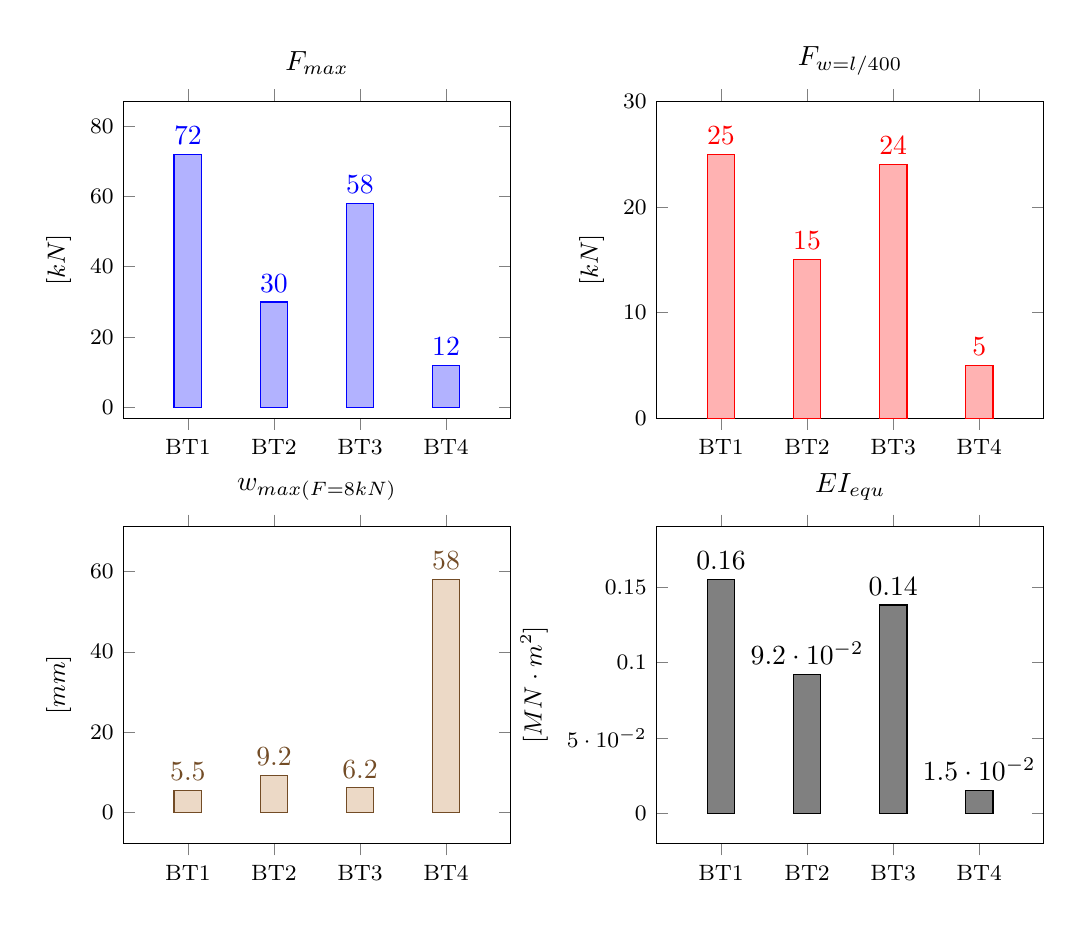
\begin{tikzpicture}
\pgfplotsset{small}
\matrix{
\begin{axis}[
			title = $F_{max}$,
			ylabel= $\lbrack kN\rbrack $,
			ybar,
			enlargelimits=0.25,
			symbolic x coords={BT1,BT2,BT3,BT4},
			xtick=data,
			nodes near coords
			]
\addplot coordinates {(BT1,72) (BT2,30) (BT3,58) (BT4,12)};
\end{axis}

&

\begin{axis}[
			title = $F_{w=l/400}$,
			ylabel= $\lbrack kN\rbrack $ ,
			ybar,
			enlargelimits=0.25,
			symbolic x coords={BT1,BT2,BT3,BT4},
			xtick=data,
			nodes near coords
			]
\pgfplotsset{cycle list shift=1}
\addplot coordinates {(BT1,25) (BT2,15) (BT3,24) (BT4,5.0)};
\end{axis}

\\

\begin{axis}[
			title = $w_{max \left( F=8kN \right) }$,
			ylabel= $\lbrack mm\rbrack $ ,
			ybar,
			enlargelimits=0.25,
			symbolic x coords={BT1,BT2,BT3,BT4},
			xtick=data,
			nodes near coords
			]
\pgfplotsset{cycle list shift=2}
\addplot coordinates {(BT1,5.5) (BT2,9.2) (BT3,6.2) (BT4,58)};
\end{axis}

&

\begin{axis}[
			title = $EI_{equ}$,
			ylabel= $\lbrack MN \cdot m^2\rbrack $ ,
			ybar,
			enlargelimits=0.25,
			symbolic x coords={BT1,BT2,BT3,BT4},
			xtick=data,
			nodes near coords
			]
\pgfplotsset{cycle list shift=3}
\addplot coordinates {(BT1,0.155) (BT2,0.092) (BT3,0.138) (BT4,0.015)};
\end{axis}

\\
};
\end{tikzpicture} 
\caption{Vergleich der Bauteilversuche (Maximallast, Durchbiegung, Biegesteifigkeit)}
\label{abb:vergleich_balkendiagramm}

\end{center}
\end{figure}

\subsubsection{Durchbiegung in Feldmitte}
In der Abbildung \ref{vergleich-durchbiegung} sind die Durchbiegungskennlinien in Trägermitte darstellt.
Es fällt auf, das die Arbeitslinien der BT1 und BT3 eine sehr gute Übereinstimmung aufweisen. Der Bauteil 2 hat eine geringere Biegesteifigkeit als diese beiden Versuchskörper. Der Träger BT\,4 hatte die geringste Biegesteifigkeit.

Um das Verformungs- und das Traglastverhalten der Sandwichbauteile zu analysieren, werden die Messwerte für eine Durchbiegung von $w=\nicefrac{l}{400}$ und eine Belastung von $F=\unit[8]{kN}$ als Vergleichswerte herangezogen. Der Wert für die Durchbiegung wurde so gewählt, dass Reserven für Langzeitverformungen gegeben sind. Der Belastungswert ergibt sich aus der Summe der Eigenlast und einer üblichen Nutzlast im Wohn- und Bürobau (Tabelle \ref{tab:vergleich_versuche} und Abbildung \ref{abb:vergleich_balkendiagramm}).

Die Maximallast verhält sich analog zu den Biegesteifigkeiten. Die Bauteile mit höherer Biegesteifigkeit $EI_{equ}$ haben auch eine höhere Maximallast $F_{max}$. 

Die Werte $w_{max, F=\unit[8]{kN}}$ und $EI_{equ}$ für den Bauteil BT\,4 weichen stark von den restlichen Werten ab, weil der Bauteil in diesem Zustand bereits versagt.

\subsubsection{Schubverformung}
Abbildung \ref{vergleich-schubverformung} vergleicht die Relativverschiebungen zwischen Beton und Holz in Abhängigkeit der Kraft an beiden Auflagern aller Bauteilversuche. Da die Verbundsteifigkeit der Schichten zwischen Beton und Holz entscheidenden Einfluss auf das Verformungs- und Tragverhalten des Sandwichbauteils hat, ist die Biegesteifigkeit der Systeme mit geringer Schubverformung am höchsten.
Dieser Zusammenhang wird auch durch die Anwendung des $\gamma$-Verfahrens als Berechnungsmodell anschaulich dargestellt (Abschnitt ????). 

\clearpage
\section{Schubversuch}
\label{abs:schubversuch}

Wie im vorigen Abschnitt erläutert, hat das Schubverhalten der Zwischenschichten zwischen Beton und Holzschicht großen Einfluss sowohl auf die Verteilung der Schnittgrößen, als auch auf das Verformungsverhalten des Sandwichbauteils.

Mit den Versuchen, die dieser Abschnitt beschreibt, kann das Schubverhalten des Systems erforscht werden.

Bei Versuchskörper BT\,1 fand das Versagen zwischen Auflager A und Lasteinleitung $F_A$ statt. In der Nähe der Lasteinleitung brach die BSP-Platte vollständig durch. Der Rest des Trägers von Lasteinleitungspunkt $F_A$ bis Auflager B hatte keine sichtbare Schädigung.

In Anlehnung an die Schubversuche in ????Literatur wurden die Versuche geplant. Für die Probekörper wurden Abschnitte des Trägers BT\,1 gewählt, in denen sich jeweils drei Schraubenpaare befanden. Mit Hilfe einer Motorsäge und einer Flex (Trennschleifer) wurde der restliche Träger zerteilt.
In Abbildung \ref{träger_scherversuch} ist ersichtlich, welche Teile des Trägers verwendet wurden. 



\begin{figure}[h]
\begin{center}
\includegraphics[scale =0.8,trim= 1cm 12cm 1cm 12cm, clip=true]{Auswertung/schubversuch/Teile_Schubversuch.pdf}
\caption{Darstellung des verwendeten Teiles der Trägers}
\label{träger_scherversuch}
\end{center}
\end{figure}



Aus ???LitVerweis
\begin{quote}
Hinsichtlich der Ermittlung von Scher- bzw. Schubfestigkeiten für den Baustoff Holz
existiert die Problematik, dass es nahezu unmöglich ist, einen reinen Schubspannungszustand
für Scherflächen parallel zur Faser zu erzeugen. Bereits Petermann
[Pet41] und Kollmann [Kol82] erkannten dieses Problem und betrachteten verschiedene
Ansätze zur Lösung desselben. Bis heute - weitere 70 Jahre nach Erscheinen der
oben genannten Arbeiten - ist diese Problematik nicht abschließend gelöst.

Im Wesentlichen haben sich heute zwei Prüfverfahren zur Ermittlung der Schubfestigkeit
von Holz etabliert, welche den einschlägigen Normen in verschiedenen Ländern
zugrunde liegen. Im Europäischen Raum bezieht sich der [DIN EN 1995-1-1] auf die
[DIN EN 408] wo das in Abbildung \ref{versuchsschema_scherversuch} dargestellte Prüfverfahren festgelegt ist. [vgl. ..........]

\end{quote}

Abbildung \ref{abb:Skizze des Schubversuchs} zeigt den abgeleiteten Versuchskörper und die Versuchsanordnung.



\begin{figure}[h!]
\begin{minipage}[hbt]{7cm}
	\includegraphics[width=7cm]{Auswertung/1versuch/versuchsschema_scherversuch.png}
	\caption{Versuchsschema: Scherversuch nach []}
	\label{versuchsschema_scherversuch}
\end{minipage}
\hfill
\begin{minipage}[hbt]{7cm}
\includegraphics[scale=1.2, trim=4cm 12cm 11.5cm 9cm, clip=true]{Auswertung/schubversuch/Schubversuch_Skizze.pdf}
	\caption{Skizze des Schubversuchs}
	\label{abb:Skizze des Schubversuchs}
\end{minipage}
\end{figure}


\subsubsection{Versuchskörper}

Folgende Schubversuche wurden durchgeführt:

\begin{enumerate}
\item Schubversuch 1 (SV\,1): 100\,x\,50\,x\,32,8\,cm
\item Schubversuch 2 (SV\,2): 150\,x\,50\,x\,32,8\,cm
\end{enumerate}

Abbildung \ref{abb: Zeichnung Schuberversuche} enthält Zeichnungen der beiden Versuchskörper.

	
	
\subsubsection{Versuchsaufbau und Messeinrichtung}
 
Der Versuchsaufbau kann der Abbildung \ref{Darstellung des Scherversuchs} entnommen werden. Der Versuchskörper wird so platziert, dass die Lasteinleitung vertikal über dem Auflager liegt. Damit der Versuchskörper die schräge Lage einnimmt, wurden Holzprofile angefertigt. Diese wurden mit Klemmzangen befestigt, um ein Ausweichen des unteren Auflagers zu verhindern.

Für die Lasteinleitung wurde ebenfalls ein Holzprofil hergestellt.

Es wurden für den Versuch zwei Messuhren (Abbildung \ref{abb:messeinrichtung_scherversuch}) am oberen Punkt des Bauteils mittels einer Stahlplatte angebracht. Somit konnte die Relativverschiebung zwischen der BSP-Schicht und der Betonschicht gemessen werden.


\begin{figure}[h!]
\begin{minipage}[hbt]{7cm}	
	\includegraphics[width=7cm]{Auswertung/1versuch/versuchsdarstellung_scherversuch_real.png}
	\caption{Darstellung des Scherversuchs}
	\label{Darstellung des Scherversuchs}
\end{minipage}
\hfill
\begin{minipage}[hbt]{7cm}	
\begin{center}
	\includegraphics[width=6cm, trim=11cm 12cm 4cm 9cm, clip=true]{Auswertung/schubversuch/Schubversuch_Skizze.pdf}
	\end{center}
    \caption{Anordnung der Messmittel }
	\label{abb:messeinrichtung_scherversuch}
\end{minipage}
\end{figure}

\subsubsection{Versuchsablauf}
Zu Beginn des Versuchs wurde eine Referenzkraft von \unit[0,5]{kN} aufgebracht. Die Messuhren wurden anschließend auf Null zurückgestellt.
Der Versuch wurde manuell kraftgesteuert durchgeführt, die Belastungsgeschwindigkeit betrug etwa \unitfrac[0,1]{kN}{s}.

Nach einem deutlichen Lastabfall wurden die Messuhren abgenommen, um eine Beschädigung der Instrumente zu verhindern.
Nach der Maximallast von \unit[359]{kN} bei Versuch SV\,1 bzw.\ \unit[348]{kN} bei SV\,2 wurde bis zum kompletten Abscheren der Betonschicht weiter belastet.

\subsubsection{Versagensbeschreibung}
\paragraph{SV\,1} 
Der Bruch deutete sich nur durch den Lastabfall an, visuell waren vor dem Bruch keine Schäden festzustellen. 

Es wurden alle Schrauben aus dem Holz herausgezogen. Das Versagen in der Holzleichtbetonschicht trat in der untersten Klebefuge ein (Abblidung \ref{abb:SV_Bruchbild_Oberfläche}). 

\paragraph{SV\,2}
Der Bruch verlief wie beim ersten Versuch.

Es wurden drei Schrauben aus dem Holz herausgezogen, die anderen drei brachen in der Holzleichtbetonschicht. Die beiden Schrauben am oberen Ende des Versuchskörpers rissen in der mittleren Velox-Schicht, während die dritte Schraube in der untersten Velox-Schicht brach.

Der Bruchverlauf in der Velox-Schicht folgt den Bruchstellen der Schrauben (Abbildung \ref{abb:bruchbild_scherversuch}). 

\subsubsection{Verformungsverhalten}
In Abbildung \ref{abb:Scherversuch Kraft Verschiebungslinie} sind die Arbeitslinien der Versuche dargestellt.

\paragraph{SV\,1}
Die unterschiedliche Verschiebung bei den beiden Messpunkten zeigt, dass sich die Betonschicht während des Versuchs verdreht hat.
Die Kurve verläuft bis zu einer Last von \unit[250]{kN} linear, danach flacht die Kurve bis zum Bruch zunehmend ab.

\paragraph{SV\,2}
Der lineare Verlauf der Kurve geht bis etwa \unit[200]{kN}. Danach entstand ein ausgeprägtes Fließplateau bei \unit[225]{kN} und schließlich nahm die Verformung progressiv zu bis zum Bruch.

Obwohl die Arbeitslinien anfangs sehr unterschiedliche Steigungen aufweisen und das Fließplateau beim ersten Versuch überhaupt fehlt, ist das Verhalten vor dem Bruch (ab \unit[230]{kN}) sehr ähnlich (Abbildung \ref{abb:VergleichSchubersuch230}).

\subsubsection{Zusammenfassung}


\begin{figure}[h!]
\begin{center}

\begin{tikzpicture}

\begin{axis}[height=12cm, width=12cm, 
			no markers,
			xmajorgrids,ymajorgrids,
			xlabel=Verschiebung\,u\,$\lbrack mm \rbrack $,
			ylabel=Kraft\,/\,Zylinder\,$\lbrack kN\rbrack $,
			xmin=0,ymin=0,
			legend pos= south east
			]
\addplot table[y=F,x=1Versuch_u1]{Auswertung/1versuch/BT1_Schubversuch.dat};
\addplot table[y=F,x=1Versuch_u2]{Auswertung/1versuch/BT1_Schubversuch.dat};
\addplot table[y=F,x=2Versuch_u1]{Auswertung/1versuch/BT1_Schubversuch.dat};
\addplot table[y=F,x=2Versuch_u2]{Auswertung/1versuch/BT1_Schubversuch.dat};
\legend{SV\,1\,u1, SV\,1\,u2, SV\,2\,u1, SV\,2\,u2}
\end{axis}
\end{tikzpicture}
\caption{Schubversuche: Kraft-Verformung}
\label{abb:Scherversuch Kraft Verschiebungslinie}
\end{center}
\end{figure}




\begin{figure}[h!]
\begin{minipage}[hbt]{7cm}	
	\includegraphics[width=7cm]{Auswertung/1versuch/bruchbild1_scherversuch.png}
	\caption{Bruchbild des Scherversuch zw. BSP- und Veloxschicht}
	\label{abb:SV_Bruchbild_Oberfläche}
\end{minipage}
\hfill
\begin{minipage}[hbt]{7cm}
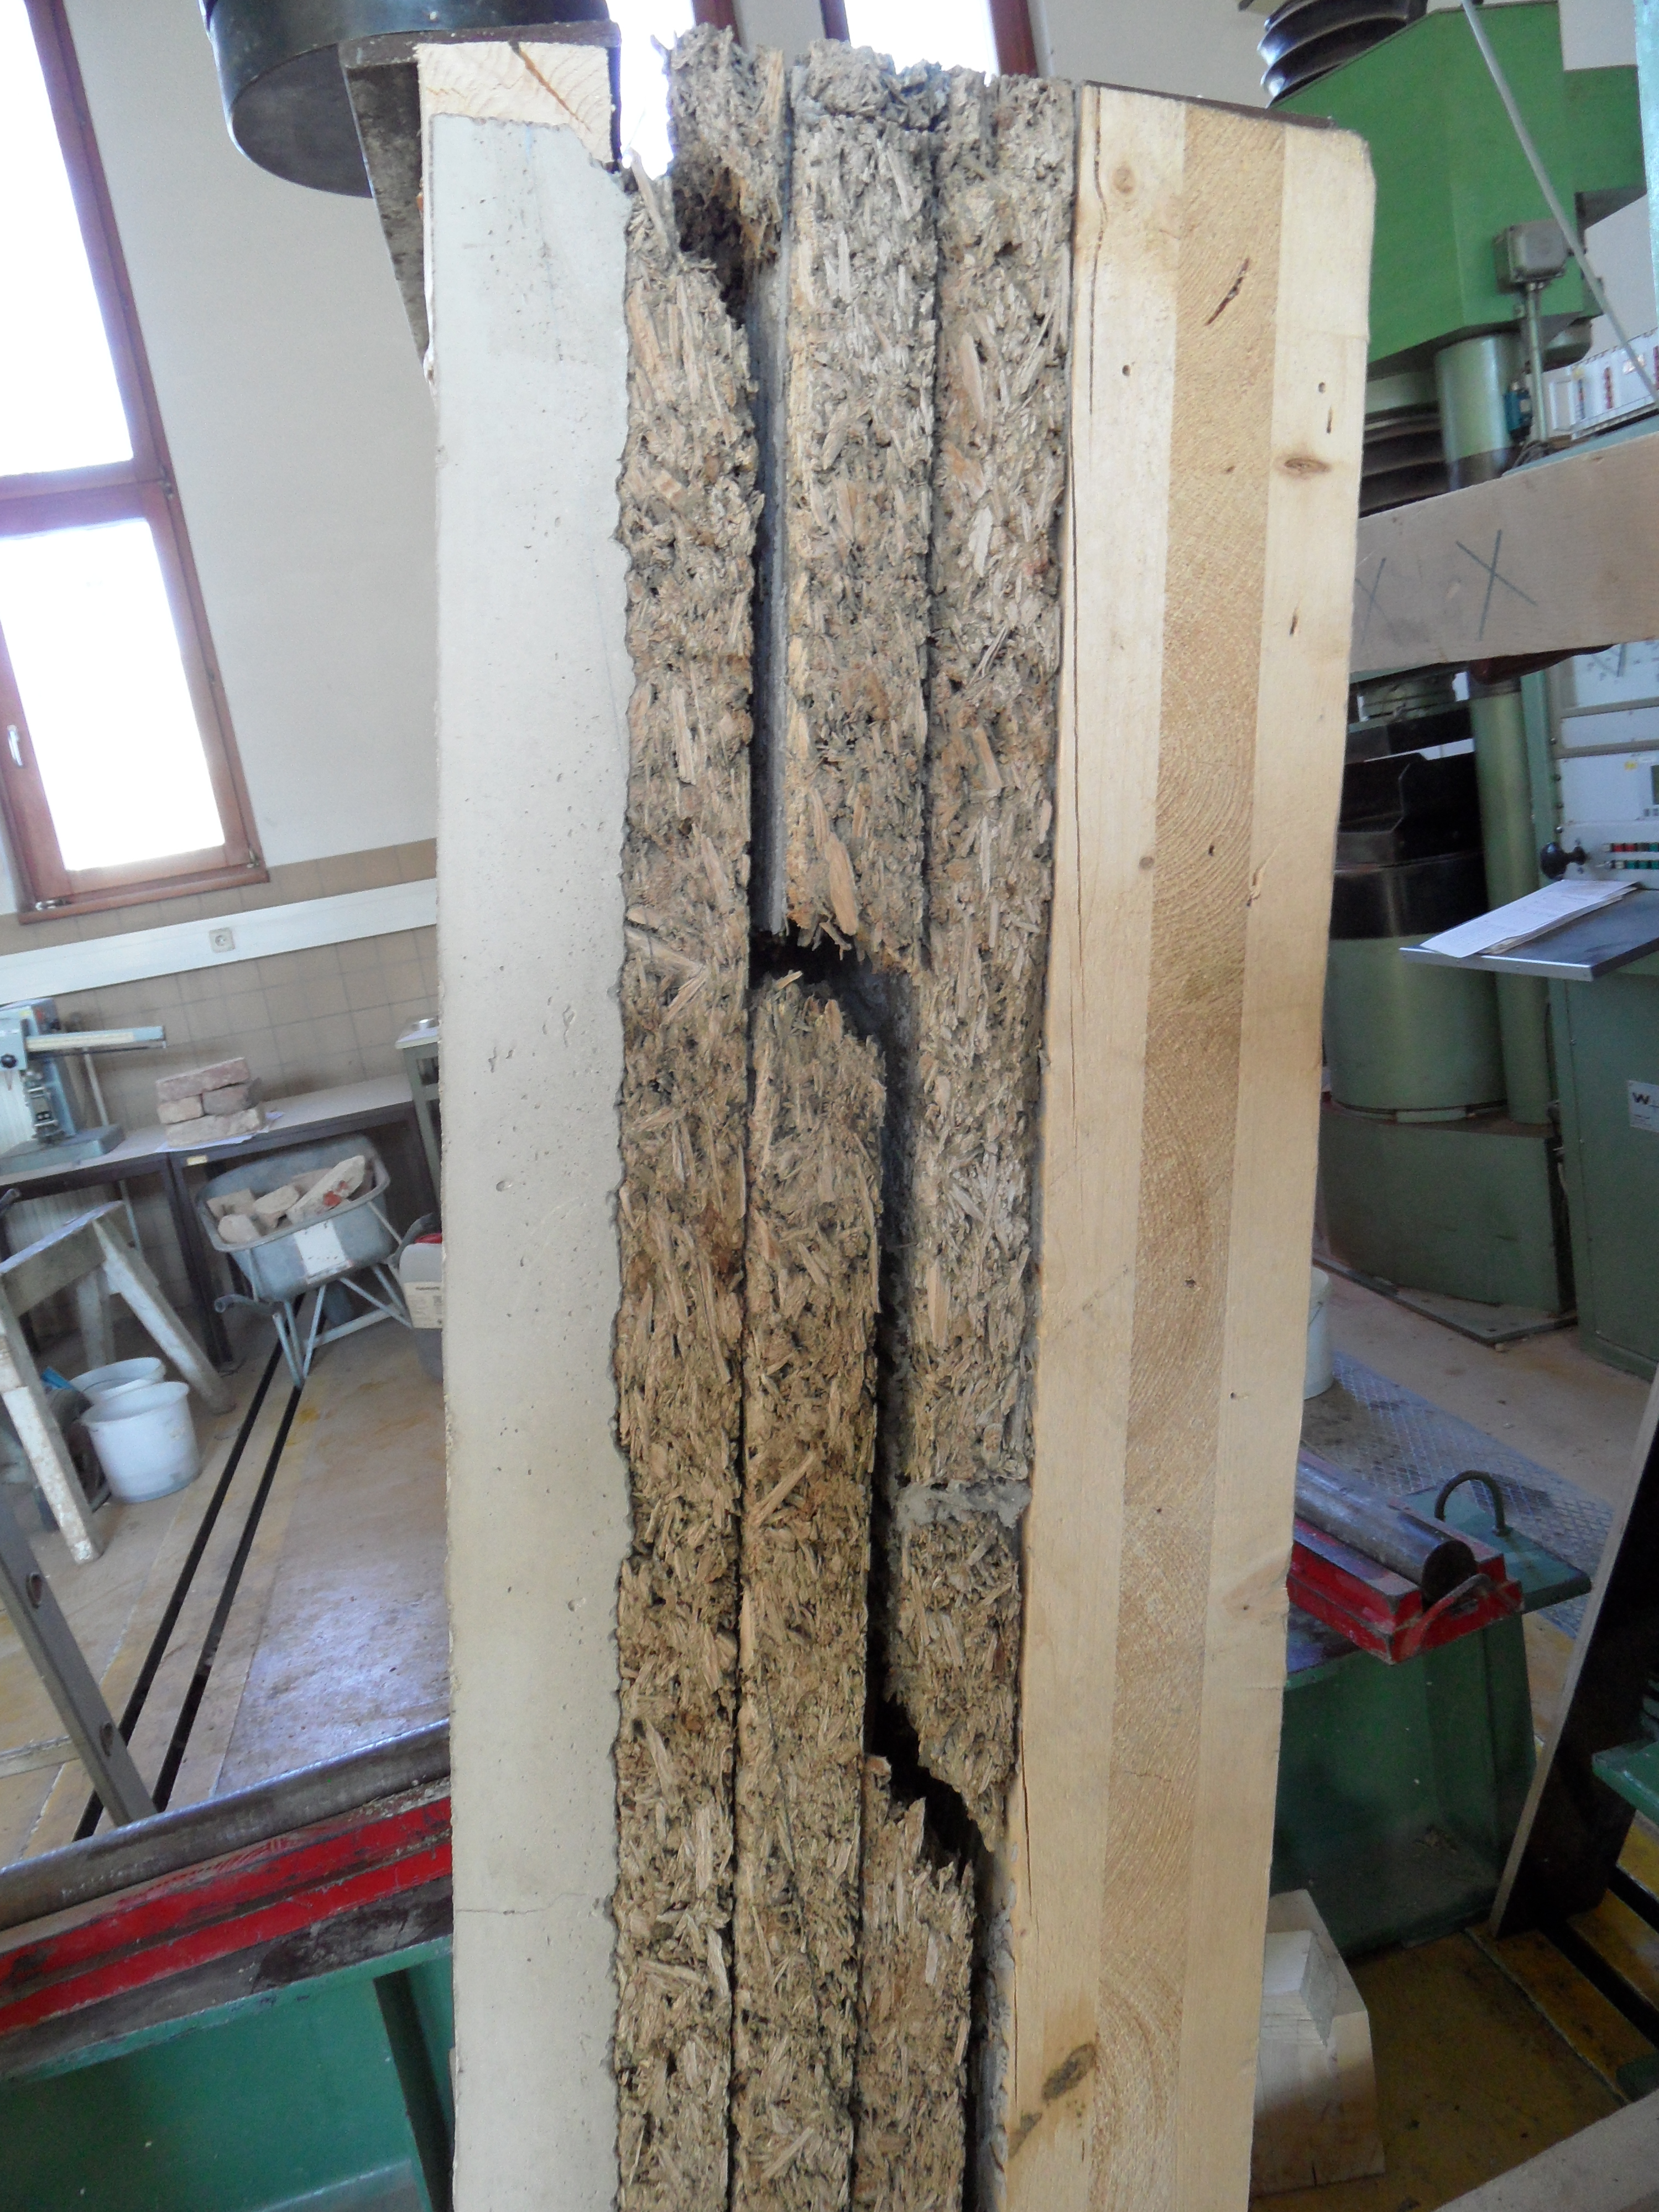
\includegraphics[width=7cm]{Auswertung/schubversuch/SV_Bruchbild_seitlich.jpg}
	\caption{SV2: seitliches Versagensdarstellung nach Bruch}
	\label{abb:bruchbild_scherversuch}
\end{minipage}
\end{figure}


\begin{figure}[h!]
\begin{center}

\begin{tikzpicture}

\begin{axis}[height=12cm, width=12cm, 
			no markers,
			xmajorgrids,ymajorgrids,
			xlabel=Verschiebung\,u\,$\lbrack mm \rbrack $,
			ylabel=Kraft\,/\,Zylinder\,$\lbrack kN\rbrack $,
			xmin=0,ymin=0,
			legend pos= south east
			]
\addplot table[y=F1,x=V1]{Auswertung/1versuch/BT1_Schubversuch.dat};
\addplot table[y=F1,x=V2]{Auswertung/1versuch/BT1_Schubversuch.dat};
\legend{SV\,1\,Mittelwert,SV\,2\,Mittelwert}
\end{axis}
\end{tikzpicture}
\caption{Vergleich der Kennlinien nach 230\,kN}
\label{abb:VergleichSchubersuch230}
\end{center}
\end{figure}




\subsubsection{Zusammenfassung}

\begin{table}[h]
\caption{Berechnung}
\begin{center}
\begin{tabular}{|c|c|c|c|c|}

\hline 
Versuch & $F_{max}$  & $F_{04}$ & $v_{04}$ & $k_{s,04}$  \\ 

&  [kN] & [kN] & [mm] & [N/mm]    \\ 
\hline\hline
SV1 & 359  & 144 & 1,17 & 123076    \\ 
\hline 
SV2 & 348  & 139 & 0,11 & 1263636   \\ 

\hline 
\end{tabular} 
\end{center}
\label{tab:Schubversuche}
\end{table}

Wie in der Einleitung dieses Abschnitts beschrieben, ist das Bauteilverhalten stark von der Verbindungssteifigkeit der Beton- mit der Holzschicht abhängig. Diese Steifigkeit wird mit dem Verschiebungsmodul $k_{s}$ beschrieben \cite{DINEN26891}.

Tabelle \ref{tab:Schubversuche} beinhaltet die Anfangsverschiebungsmodule $k_{s,04}$ für eine Belastung von $0,4 \cdot F_{max}$.

\begin{equation}
k_{s,04} = \dfrac{F_{04}}{v_{04}}
\end{equation}

\begin{itemize}
\item $F_{04} = 0,4 \cdot F_{max}$
\item $v_{04}$ \ldots Verschiebung bei $F_{04}$
\end{itemize}

Es zeigt sich, dass der Verschiebungsmodul des Versuchs SV\,2 das zehnfache des Ergebnisses aus dem Versuch SV\,1 beträgt. Durch die undefinierte Vorbelastung durch den Versuchsablauf und die darauf folgende Manipulation (Lagerung und Bearbeitung des Trägers) kann ohne weitere experimentelle Untersuchungen keine Interpretation der stark streuenden Ergebnisse getroffen werden.

Diese Untersuchungen sind im Rahmen des Forschungsprojektes `"Titel blalalalalala (Ali fragen)'" vorgesehen.




\clearpage

\section{Conclusio und Ausblick}
\subsection{Conclusio}
\subsubsection{Biegeversuche}
\paragraph{Lastfall Montage und Transport}
Das statische System der durchgeführten Biegeversuche ist ein Einfeldträger mit zwei Einzellasten in den Viertel-Punkten. Im Montage- und Transportzuständen können jedoch andere statische Systeme auftreten, welche beim Entwurf der Elemente berücksichtigt werden müssen. Das zeigten insbesondere die Versuche BT\,2 und BT\,4  (Abschnitt \ref{abs:BT2_Schaden} und \ref{abs:BT4_Schaden}). Dieses Problem kann durch eine entsprechende Anordnung der mechanischen Verbindungsmittel vermieden werden (siehe Versuchskörper BT3, Abschnitt \ref{abs:BT3_Versuchskoerper}). 

\paragraph{Herstellung der Klebefuge}
Die Bauteilversuche zeigten, dass folgende Kriterien Einfluss auf die Qualität der Klebefugen hatten. 

Eine gute \textit{Verarbeitbarkeit} des Klebers ermöglicht ein gleichmäßiges und rasches Auftragen der Klebemasse auf den Untergrund. Die Verarbeitbarkeit hängt von der Viskosität des Klebers ab. Je flüssiger der Kleber, desto leichter die Verarbeitung. Jedoch müssen beim Auftragen mit der Zahnspachtel die Riefen stehen bleiben. 

Die \textit{Klebermenge} ist entscheidend für eine vollständig Vernetzung der zu verbindenden Schichten. %(Abschnitt \ref{abs:Klebeversuch_Menge}!!!!!!!!!)

Die Vorverformung (Aufschüsseln durch Lagerung) der Velox-Platten muss bei der Wahl der Klebermenge und beim Verlegen der Platten berücksichtigt werden, um eine vollständige Vernetzung zu gewährleisten.

\paragraph{Anordnung mechanischer Verbindungsmittel}

Die Verankerung der Schrauben im Beton hielt den Belastungen stand. 
Bei keinem Versuch wurden Schrauben aus dem Beton ausgezogen. 

Das Versagen der Schrauben trat entweder durch Herausziehen aus dem Holz oder durch den Bruch in der untersten Klebefuge ein.

Wie eingangs beschrieben dienen die Schrauben im Auflagerbereich auch der Aufnahme der Schubkräfte beim Lastfall Transport.

Die Anzahl der verbauten Schrauben unterscheidet sich bei den beiden Versuchen BT\,3 (6 Schrauben je Schraubenreihe) und BT\,1 (14 Schrauben je Schraubenreihe) stark. Das Verformungsverhalten war jedoch sehr ähnlich (Abbildung \ref{Vergleich_durchbiegung}). Unter der Lastanordnung in den Biegeversuchen tragen die Schrauben zwischen den beiden Lasteinleitungspunkten wenig zur Biegesteifigkeit des Sandwichträgers bei.

Die Vorschädigungen beim BT\,4 (\ref{}) zeigen, dass das Fehlen der Schrauben die Qualität der Verbundfuge negativ beeinflusst. Bei Bauteil 3 konnte durch Verwendung von Schrauben das Aufgehen der Klebefugen während dem Aushärten verhindert werden.

\paragraph{Beton}

Der selbstverdichtende Beton ging einen guten Verbund mit dem porösen Werkstoff Velox ein. In keinem Versuch versagte diese Fuge. 

\subsubsection{Schubversuche}
Aus den durchgeführten Versuchen kann wegen der Vorbelastung aus den Biegeversuchen kein eindeutiges Schubverformungsverhalten abgeleitet werden (Abschnitt \ref{abs:schubversuch}). 

\subsection{Ausblick}

Es sind weitere Schubversuche notwendig, um Berechnungsparameter ($k_s$) für die Berechnungsmethoden in Abhängigkeit der verwendeten Materialien (z.B.\ Schubmodul von Holzleichtbeton und Anzahl der Schrauben) zu bestimmen und um die Bemessungsmodelle zu konkretisieren. Es sollen Erkenntnisse zur Anzahl, Anordnung und Geometrie der Schrauben gewonnen werden. 

Es sollten Langzeitversuche durchgeführt werden, um das Kriechverhalten des Systems, sowie das Langzeitverhalten von Holzleichtbeton in Zusammenspiel mit den Verbindungsmittel (Schrauben und Kleber) zu untersuchen.

Die Anwendung als Durchlaufträger wurde nicht berücksichtigt. Durch das Auftreten eines negativen Moments, kehren sich Druck- und Zugzone um. Für die Aufnahme der Zugkräfte im Beton sind Bewehrungseinlagen notwendig. Die Anordnung der Schrauben muss an das statische System angepasst werden. Dabei ist zu berücksichtigen, dass die Schrauben unter Druckbelastung ausknicken können.

Details im Auflagerbereich und im Bereich der Fugen zwischen den vorgefertigten Elementen müssen entwickelt werden. Aus statischer Sicht muss die Scheibenwirkung der gesamten Decke (Abtragen von Horizontallasten) und die Querkraftübertragung zwischen den Elementen gewährleistet sein.


Fertigungsprozess (Fertig-Teilfertigteil)???? 














	
	
